%----------------------------------------------------------------------------
\chapter{Design}
\label{cha:design}
%----------------------------------------------------------------------------

In this chapter I will present the design phase of a new model based testing framework, that tries to take into consideration of the conclusions of the investigated available testing tools. This framework is need to be complete regarding the whole MBT process, and has to help in all phases of the testing. The different phases will be discussed separately as at the model based testing process specification (Section \cite{sec:process}).

\begin{enumerate}

\item The first step is the creation of the model. There are many possibility to choose from and we want to have a transition based notation that represents some kind of state machine. State machine notations have different level of expression and come with different amount of features. Generally the more feature a modelling language has, the more hard to generate a good quality test suite from it. That's why we need to find a notation that has a suitable level of expressiveness and it is easy to integrate into a complete testing process.

Earlier we saw that the lowest level of state machine notation is some kind of FSM like notation. However FSMs lacks of many features and a real world software is hard to model with it. Actions, guards, events are not even parts of the improved EFSM notation, so we need to find something more expressive.

Many tools have an UML like notation, but they either can not fully take advantage of the many features of this modelling language or simply avoid their usage. That is not surprising because UML was not designed for testing purposes. UML has just all the features, that are needed to describe the behaviour of a real life software, but some of its feature are hard to utilise during the test generation process. Moreover it lacks some important feature, that a test model has to bear with.

It would be ideal if the test model would express the output of the state machine, because determining the expected output would be trivial by the test generation process. However an UML like semantics and syntax would be easy to adopt by the test engineers, because UML state machines are well known in the industry field and most of its features are easy to use and self-describing. Unfortunately the UML modelling language has lot of implementation and they differ in terms of integrability.

For these issues noted above I think a solution can be the Eclipse Modeling Framework. It is a modelling framework that is built especially for creating tools based on structured models. As the most important advantages of using EMF help with the implementation, it will be discussed in more details in Chapter~{cha:implementation}.

EMF models are easy to use, extendable models, that have an UML like syntax.  These models are customisable for the actual needs, and suitable meta-model can be built with the help of the EMF platform. PLCspecif is complete solution that has exactly these previously defined features.

\section{PLCspecif}
\label{sec:plcspecif}

PLCspecif is a modelling language intended to be a formal, modular, hierarchical behaviour specification method for describing PLC programs. It was created as part of a doctoral programme by Dániel Darvas of the Budapest University of Technology and Economics (BUTE) and the European Organization for Nuclear Research (CERN).

The abstract syntax of the PLCspecif formalism was designed as an EMF metamodel, therefore the figures are following the original EMF denotation. Here I will describe only the concerned parts of the modelling language as the complete feature set goes far beyond this thesis.

\begin{figure}[htp]
\centering
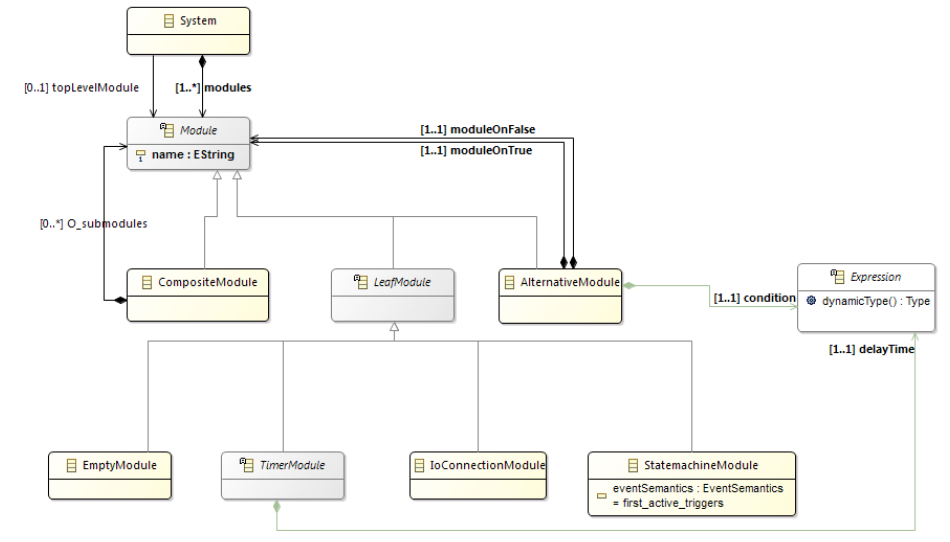
\includegraphics[scale=0.4]{figures/plchsm_modules}
\caption{Module structure of PLCspecif}
\label{fig:plchsm_modules}
\end{figure}

The specification organised into modules (Figure~\ref{fig:plchsm_modules}), which are either represent a behaviour of concrete module (\texttt{LeafModule}) or they are composite modules containing a set of submodules (\texttt{CompositeModule}).

\texttt{System} is a top-level container that can contain \texttt{modules} from which one module represents the \texttt{topLevelModule}. There are four different module type:

\begin{itemize}
	\item \texttt{StatemachineModule} represents an UML-like state machine.
	\item \texttt{IoConnectionModule} defined by connections between input and output variables.
	\item \texttt{TimerModule} describes a PLC timer in the system.
	\item \texttt{EmptyModule} is a module without any state machine or IO connection.
\end{itemize}

From these module types we are interested especially in the state machine notation. As shown on Figure~\ref{fig:plchsm_statemachine} the metamodel is similar to UML state machine's metamodel described previously (Subsection~\cite{ssub:umlstatemachine}).

\begin{figure}[htp]
\centering
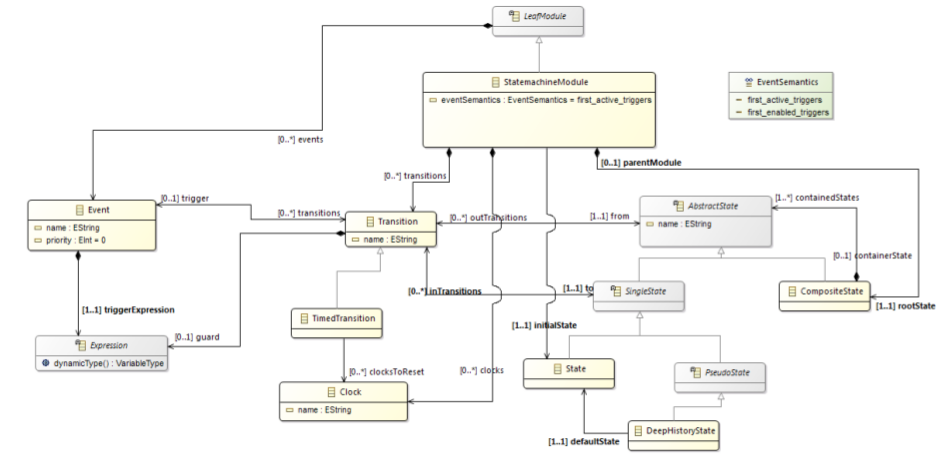
\includegraphics[scale=0.5]{figures/plchsm_statemachine}
\caption{Structure of \texttt{StatemachineModule}}
\label{fig:plchsm_statemachine}
\end{figure}

On the other hand PLCspecif state machines have some differences from the UML notation:

\begin{itemize}
	\item There is a root state, that recursively contains all of states.
	\item There are pseudo states (\texttt{DeepHistoryState}), which can save a state configuration for its container state.
	\item There are \texttt{TimedTransitions}, which are transitions having time-related conditions.
	\item With \texttt{Clocks} it is possible to define synchronous stopwatches, which can measure the elapsed time since last reset.
	\item Parallel regions are not allowed.
	\item Initial state can not be defined for composite states.
	\item At every moment, exactly one atomic state can be active. 
\end{itemize}

Beside these differences PLCspecif has a bigger difference, which can improve the usability of a test model. Modules can handle input and output variables and can define their outputs using \texttt{VariableDefinitionExpression} objects (Figure~\cite{fig:plchsm_variables}). PLCspecif offers a wide range of possibilities to define an \texttt{Expression}, e.g. \texttt{SwitchCaseTable}, \texttt{DnfExpression}, \texttt{Contant}, \texttt{UnaryOperation}, \texttt{BinaryOperation}, \texttt{NaryOperation}. In our case the output definition of a single state machine can be a switch case table, where conditions checks whether the state machine is in a particular state, and the values are the possible values given by a variable or constant.

\begin{figure}[htp]
\centering
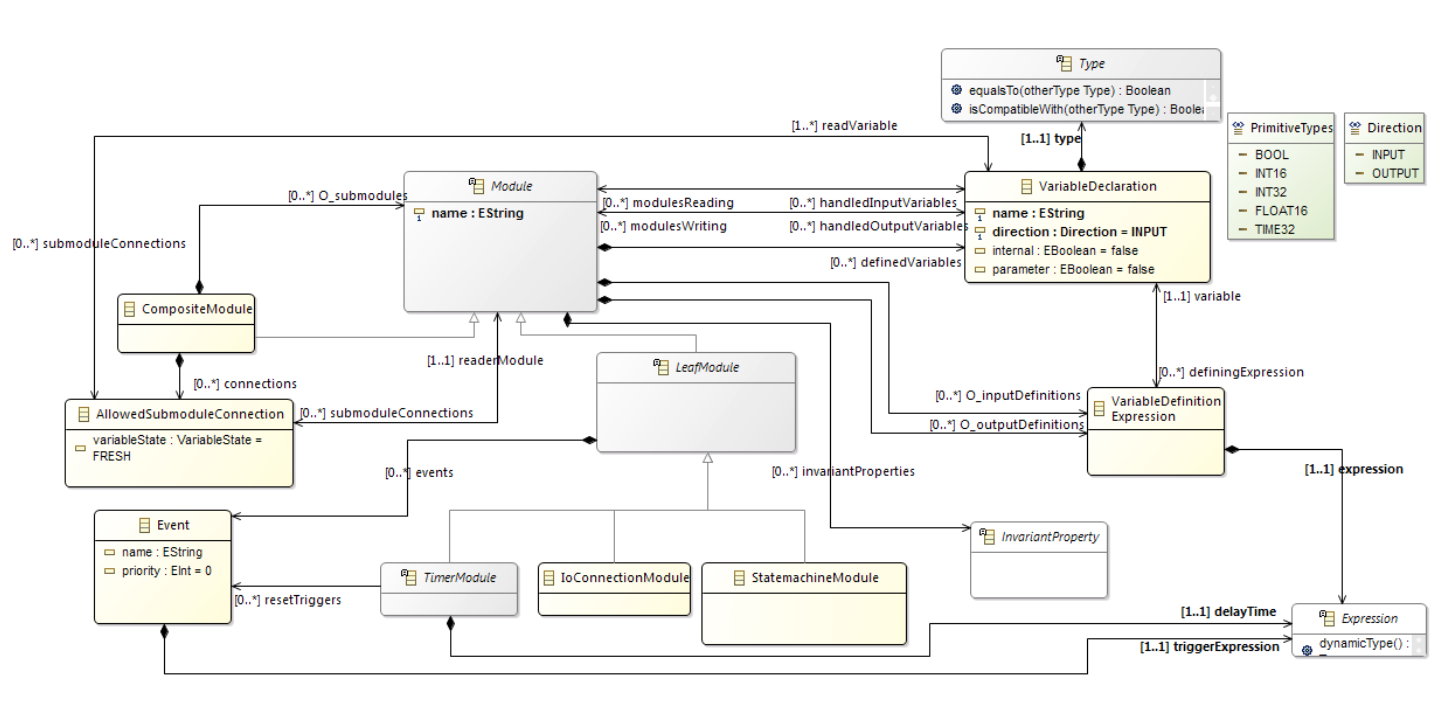
\includegraphics[scale=0.5]{figures/plchsm_variables}
\caption{Variables in PLCspecif}
\label{fig:plchsm_variables}
\end{figure}

We can see, that PLCspecif has some advantage over traditional UML modelling language in the field of model based testing:

\begin{itemize}
	\item EMF Ecore is a reference implementation of OMG's Essential Meta-Object Facility, that's why syntax should conform with the original UML denotation.
	\item PLCspecif is rather a subset of the UML state machine language, and so it is more simple.
	\item PLCspecif is able to express natively the outputs of a state machine, which can be utilised greatly by the test case generation.
	\item As PLCspecif is based on the EMF Ecore metamodel engineers can take advantage of the entire EMF ecosystem and tooling by the whole MBT process.
	\item UML language has only an informally given semantics, while PLCspecif has a complete formal behaviour specification.
\end{itemize}

% section plcspecif (end)

\item The next step of model based testing is the test planning.

The scope of a generated test suite is always is referred to the corresponding state machine. In reality following the Law of Demeter and decoupling, that would mean one class or two classes.

Another important question to discuss is the specification of chosen test selection criteria. We saw at the conclusions of the investigation of related works (Chapter~\cite{cha:relatedwork}), that even the most general and simplest criteria are not fully supported by all the available tools. They either implement complex criteria with a less useful, simple model, or they work with an expressive model and do not support the criteria completely.

At this point I tried to find a golden mean between the different approaches. I chose to implement the basic structural model coverage criteria (full state and transition coverage) on a model with moderate level of expressiveness. Formalisation of this criteria is mostly trivial and left to the implementation chapter (\cite{cha:implementation}).
\item ... % TODO: test case generation

\section{Alloy}
\label{sec:alloy}

Alloy is a formal modelling language to define structures. Alloy can be utilised with a tool, called Alloy Analyzer to automate the verification process. The tool transforms problems into SAT formulas to solve them. The solver was inspired by model checkers, but it is implemented as a constraint solver, performing verification within a bounded scope.

The strength of this tool allows us to define our test generation goals with the Alloy language to generate the test cases. The test cases need to guarantee state-based and transition-based coverages.

% section alloy (end)

\item ... % TODO: test execution

\end{enumerate}

% chapter design (end)